% ------------------------------------------------------------------------
% file `revisions_juin-exercise-32-exercise-body.tex'
%   in folder `xsim/'
%
%     exercise of type `exercise' with id `32'
%
% generated by the `exercise' environment of the
%   `xsim' package v0.20c (2021/02/03)
% from source `revisions_juin' on 2023/06/06 on line 564
% ------------------------------------------------------------------------
	Un étang circulaire de 4 m de rayon est bordé par une allée de 2 m de large, le tout étant clôturé par un treillis.
	\begin{multicols}{2}
		\begin{enumerate}
			\item \emph{(Sur cette feuille)} Indique les données du problème sur la figure ci-contre. %pourquoi c'est souligné?
			\item \emph{(Sur cette feuille)} Hachure la surface de l’allée.
			\item Calcule l’aire de cette allée.
			\item Calcule la longueur du treillis.
		\end{enumerate}
		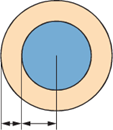
\includegraphics{img/etang.png}
	\end{multicols}
